\chapter{Problem definition: Waste material in city-regions}

Environmental degradation, miss usage of resources, and pollution are not virtual or intangible processes, they are tied to specific locations. There is a reason behind the geographical structure of these events which also deserves to be explored. By introducing the spatial dimension to the analysis, planning for better city-regions becomes spatial planning. \par

The problem of improving the quality of human settlements is complex and requires of a holistic approach to make effective contributions (Figure \ref{fig:complex_sdg}). There is a significant amount of interactions between the goals and in order to plan for a more sustainable places, these relationships need to be explored \parencite{Eurostat2019, Miola2019,euc2019}. By systematically looking at how these goals relate to each other, synergies can be enhanced, and tensions taken into consideration. Planning as a general practice will deal with evaluating and organizing what is the best course of action to meet a target. \par
%
Monitoring KPIs is an important activity, they provide information about the result of a process (or processes). By them self, they do not contain information about how a system works or is performing, but information about the working of a system are important for Planning purposes. \par
%


\begin{figure}[hbt!]
    \centering
    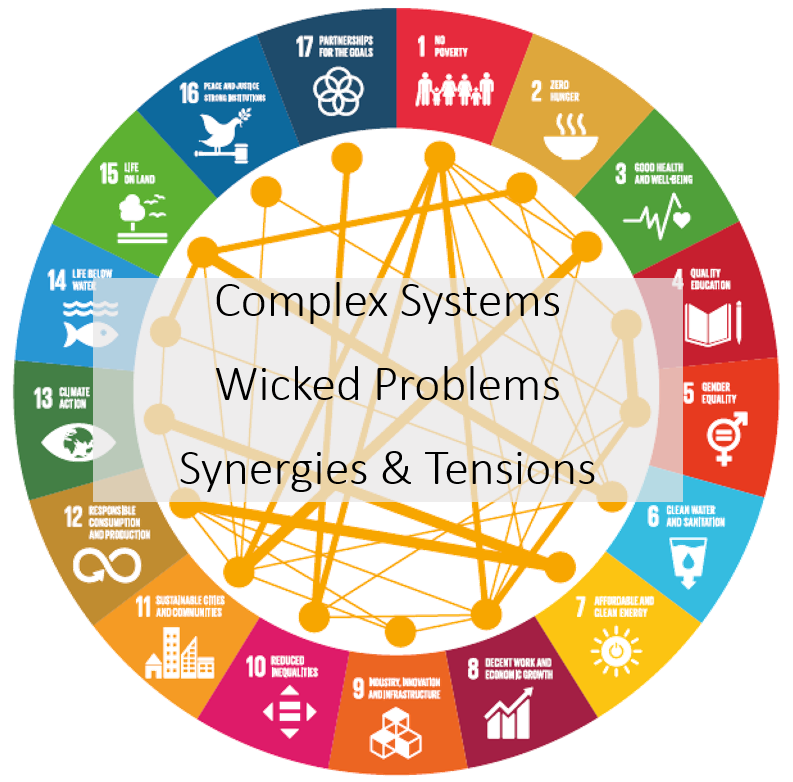
\includegraphics[width=0.45\textwidth]{sections/asset/3_complex.PNG}
    \caption{SDGs: Complex and Wicked Planning problems \parencite[pp. 30]{Eurostat2019}}
    \label{fig:complex_sdg}
\end{figure}
%

For the purpose of this exposition, the idea that a city-region works as a factory will be used to illustrate the general problem being faced here. Now, let's imagine that the owner of a factory wants to increase the production, she would start to ask questions about how much is being currently produced and then start to monitor the amount of inputs requested. By solely looking at these variables, much planning cannot be done. Decisions about the amount and the combination inputs could help to enhance production, but soon more question about the processes behind production will arise. More information about the components of the factory will be requested, number of employees, salaries, energy consumption, machines used, and so forth. As more and more detailed KPIs about the production are being monitored, the processes of production will be revealed. \par

A city is not a factory. Besides many other differences, in a factory the processes are linear. Inputs are transformed step by step in a linear process. Each step is related to the previous one and so forth. Once a part moves forward in the production line, it never goes back and affects previous process. Social and economic systems are complex and any performance indicator needs to take into account the complexity of these systems. 
In order to meet the targets, it has never been clearer that spatial planning is necessary. In some urban domains such as transport, there has been long tradition of exploring the relation between land use, mobility and socio-economic activities. As a result of data availability and it's natural proximity to geography, transport systems have been spatially planned for long time. New data sources and technological innovation can contribute to enhance the study of space in other urban domains. \par

\textcite{Rittel1973} argue that in \textit{`large and interconnected network systems(...), it has become less apparent where problem centers lie, and less apparent where and how we should intervene even if we do happen to know what aims we seek'}. Only after unpacking the systems interrelations, it would be possible to meet targets that are sustainable over time and minimize undesirable side effects.\par

Because most of these are urban or regional processes occurring in specific locations, spatial planning becomes the tool to help to define the specific set of actions in the space to affect performance.  \par

To sum up, to modify the performance of a complex system it is needed to:


\begin{enumerate}
    \item Understand the processes within the system
    \item Understand how that system interacts with other systems
    \item Understand the spatial-temporal properties 
\end{enumerate}


\section{Problem statement}


The following major issues must be considered in discussing the management of solid wastes: \parencite{CDR2005}\par

\begin{enumerate}
    \item increasing waste quantities
    \item wastes not reported in the national MSW totals
    \item lack of clear definitions for solid waste management terms and functions
    \item lack of quality data
    \item need for clear roles and leadership in federal, state, and local government
    \item need for even and predictable enforcement regulations and standards
    \item resolution of inter county, interstate, and inter country waste issues for MSW and its components
\end{enumerate}


Despite the many advantages obtainable from developing an effective recycling process, experience has shown that several barriers hinder the development of effective recycling markets \parencite{CDR2005}:

\begin{enumerate}
    \item Lack of consumer awareness about recycled products
    \item Lack of consumer confidence in the quality of products made from recycled materials
    \item The social costs and benefits are not reflected in the price of products. Despite environmental advantages, recycled products are generally more expensive than their counter- parts made from virgin materials
    \item The high cost of transporting recyclables from the point of collection in many cities and rural areas to centralized processing plants
    \item Uncertainty about supply-and-demand stability of recyclable products deters financial investment in facilities using recycled materials
    \item Recovery and sorting of certain recyclable materials such as plastics, oil, tires, and demolition products is difficult, and technological improvements are necessary to increase the efficiency of recovery.
\end{enumerate}







\section{Challenge}
The importance of the SDGs and its KPIs is recognized as a step forward to meet the global sustainability. Yet, there is a link missing between how things are done in practice (in the territory) and what the SDG indicators are addressing. This gap needs to be bridged. There is a challenge raised by SDG11, to build better human settlements, and this means dealing with space. dealing with the spatial planning of places. In order to plan better city-regions there is a need of spatializing, modelling and understanding how space (the specific location of places and events) can be adequately incorporated into valuable information for planning. \par

As described above, KPIs do not give information about the set of actions needed to create sustainable places or improve how resources can be used more efficiently. Studying and understanding the interaction between the indicators is crucial, but also where  and when in time these events happen is important and not trivial. \par

Moreover, since generally speaking these KPIs are aggregated at national levels (rarely broken down into smaller geographical units), it becomes difficult for local governments to plan for sustainable development. \par 
Finally, the metrics used to evaluate progress in sustainable development are a-spatial and do not take into consideration how different places interact or the the role of places. Since, cities are important for global sustainability, local and regional authorities need to plan better regions and the demand for metrics that can capture what is actually happening in their territories is necessary. 



\begin{figure}[h!]
    \centering
    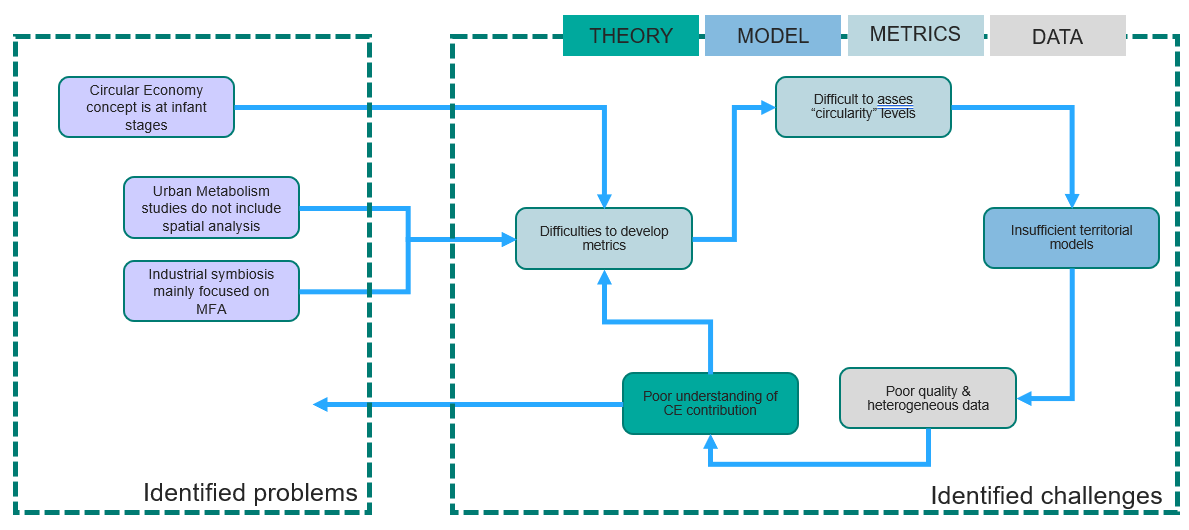
\includegraphics[width=0.8\textwidth]{sections/asset/challenge_probs.PNG}
    \caption{Problem and challenge identification}
    \label{fig:problems}
\end{figure}


